
\documentclass[24pt,a0paper,landscape]{tikzposter}


% \usepackage[x-1a]{pdfx}
\usepackage[utf8]{inputenc}
% \hypersetup{pdfencoding=unicode}
% \inputencoding{utf8}

% poster template
% $\usepackage[orientation=landscape,size=a0,scale=1.4,debug]{beamerposter}
% \usepackage{txfonts}


% \usetheme{zurichposter}
% \usepackage{fp}
 \usepackage[absolute,overlay]{textpos}

%\usepackage{natbib}
\usepackage{filecontents}
\usepackage{tabularx}
\usepackage{adjustbox}

\begin{filecontents}{poster.bib}
@InCollection{charikar2000greedy,
  Title                    = {Greedy approximation algorithms for finding dense components in a graph},
  Author                   = {Charikar, M.},
  Booktitle                = {APPROX}, 
  Year                     = {2000},
  Pages                    = {84--95},
}

@Misc{GoldbergG84,
  Title                    = {Finding a maximum density subgraph},
  Author                   = {Goldberg, A.~V.},
  howpublished                  = {Berkeley, CA},
  Year                     = {1984},
}

@Misc{jiang2009mining,
  Title                    = {Mining frequent cross-graph quasi-cliques},
  Author                   = {Jiang, D. and Pei, J.},
  howpublished                  = {KDD '09},
  Year                     = {2009},
}

@Article{li2011integrative,
  Title                    = {Integrative analysis of many weighted co-expression networks using tensor computation},
  Author                   = {Li, W. and Liu, Chun-Chi and Zhang, Tong and Li, Haifeng and Waterman, Michael S and Zhou, Xianghong Jasmine},
  Journal                  = {PLoS Comp Bio},
  Year                     = {2011},
  Number                   = {6},
  Pages                    = {e1001106},
  Volume                   = {7},
}

\end{filecontents}


% references
\usepackage[bibstyle=authoryear, citestyle=authoryear,hyperref=auto]{biblatex}
\bibliography{poster.bib}
\usepackage{tikz}


\usetikzlibrary{calc,matrix,shapes,positioning,fadings}

\tikzfading[name=fade out,
inner color=transparent!0,
outer color=transparent!100]


\newcommand{\convexpath}[2]{
[   
    create hullnodes/.code={
        \global\edef\namelist{#1}
        \foreach [count=\counter] \nodename in \namelist {
            \global\edef\numberofnodes{\counter}
            \node at (\nodename) [draw=none,name=hullnode\counter] {};
        }
        \node at (hullnode\numberofnodes) [name=hullnode0,draw=none] {};
        \pgfmathtruncatemacro\lastnumber{\numberofnodes+1}
        \node at (hullnode1) [name=hullnode\lastnumber,draw=none] {};
    },
    create hullnodes
]
($(hullnode1)!#2!-90:(hullnode0)$)
\foreach [
    evaluate=\currentnode as \previousnode using \currentnode-1,
    evaluate=\currentnode as \nextnode using \currentnode+1
    ] \currentnode in {1,...,\numberofnodes} {
-- ($(hullnode\currentnode)!#2!-90:(hullnode\previousnode)$)
  let \p1 = ($(hullnode\currentnode)!#2!-90:(hullnode\previousnode) - (hullnode\currentnode)$),
    \n1 = {atan2(\y1,\x1)}, 
    \p2 = ($(hullnode\currentnode)!#2!90:(hullnode\nextnode) - (hullnode\currentnode)$),
    \n2 = {atan2(\y2,\x2)},
    \n{delta} = {-Mod(\n1-\n2,360)}
  in 
    {arc [start angle=\n1, delta angle=\n{delta}, radius=#2]}
}
-- cycle
}


\newcommand{\nwA}[1][0.05]{\begin{tikzpicture}[remember picture]
\node {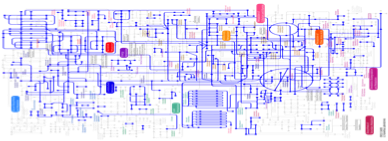
\includegraphics[height=#1\textheight]{metabolic-images/rn-network}} ; 
\end{tikzpicture}}


\newcommand{\nwB}[1][0.05]{\begin{tikzpicture}[remember picture]
\node {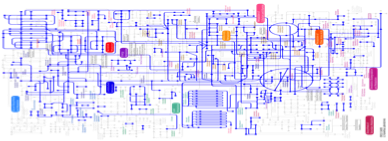
\includegraphics[height=#1\textheight]{metabolic-images/rn-network}} ; 
\fill [blue,path fading=fade out] (-0.5, -1) rectangle (0.5, 1); 
\end{tikzpicture}} 

\newcommand{\nwC}[1][0.05]{\begin{tikzpicture}[remember picture]
\node {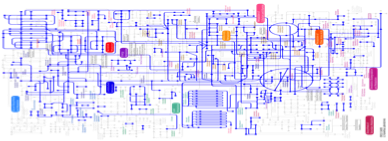
\includegraphics[height=#1\textheight]{metabolic-images/rn-network}} ; 
\fill [green,path fading=fade out] (-2.5, 0.5) rectangle (-0.5, 1.5); 
\fill [red,path fading=fade out] (0, -1.5) rectangle (1.5, 0); 
\end{tikzpicture}}

\newcommand{\gAsmall}{
\def \n {6}
\def \radius {2.0cm}
\def \margin {8} % margin in angles, depends on the radius
\foreach \s in {1,...,6}
{
{\node[draw, circle,scale=0.5] (\s) at ({360/\n * (\s - 2)}:\radius)  {\small $\s$};}
} 
\draw [color=blue,very thick] (1) -- (2) ; 
\draw [color=blue,very thick] (4) -- (2) ; 
\draw [color=blue,very thick] (1) -- (3) ; 
\draw [color=blue,very thick] (1) -- (4) ; 
\draw [color=blue,very thick] (4) -- (5) ; 
\draw [color=blue,very thick] (3) -- (5) ; 
\draw [color=blue,very thick] (6) -- (5) ; 
\draw [color=blue,very thick] (3) -- (4) ; 

}

\newcommand{\gAsmallA}{
\def \n {6}
\def \radius {2.0cm}
\def \margin {8} % margin in angles, depends on the radius
\foreach \s in {1,...,5}
{
{\node[draw, circle,scale=0.5] (\s) at ({360/\n * (\s - 2)}:\radius)  {\small $\s$};}
} 
{\node[draw, circle,scale=0.5] (6) at ({360/\n * (4)}:\radius)  {\small $\s$};}

\draw [color=blue,very thick] (1) -- (2) ; 
\draw [color=blue,very thick] (4) -- (2) ; 
\draw [color=blue,very thick] (1) -- (3) ; 
\draw [color=blue,very thick] (1) -- (4) ; 
\draw [color=blue,very thick] (4) -- (5) ; 
\draw [color=blue,very thick] (3) -- (5) ; 
\draw [color=blue,very thick] (3) -- (4) ; 
}

\newcommand{\gBsmall}{
\def \n {6}
\def \radius {2cm}
\def \margin {8} % margin in angles, depends on the radius
\foreach \s in {1,...,6}
{
\node[draw, circle] (\s) at ({360/\n * (\s - 2)}:\radius) {\small $\s$};
} 
\draw [color=red,very thick] (1) -- (2)  ; %node [near end, below=5pt] {\Large\textcolor{red}{$x^{(2)}_{12}$}}; 
\draw [color=red,very thick] (3) -- (2)  ; % node [near end, above=10pt] {\Large\textcolor{red}{$x^{(2)}_{23}$}}; 
\draw [color=red,very thick] (1) -- (3)  ; % node [midway, below=10pt] {\Large\textcolor{red}{$x^{(2)}_{13}$}}; 
\draw [color=red,very thick] (4) -- (2)  ; % node [near start, below=2pt] {\Large\textcolor{red}{$x^{(2)}_{24}$}}; 
\draw [color=red,very thick] (3) -- (4)  ; % node [midway, above=1pt] {\Large\textcolor{red}{$x^{(2)}_{34}$}}; 

\draw [color=red,very thick] (1) -- (6)  ; % node [midway, below=1pt] {\Large\textcolor{red}{$x^{(2)}_{16}$}}; 
\draw [color=red,very thick] (3) -- (6)  ; 
}

\newcommand{\gA}[1][4cm]{
\def \n {6}
\def \radius {{#1}}
\def \margin {8} % margin in angles, depends on the radius
\foreach \s in {1,...,6}
{
{\node[draw, circle] (\s) at ({360/\n * (\s - 2)}:\radius)  {\small $\s$};}
} 
\draw [color=blue,very thick] (1) -- (2) ; 
\draw [color=blue,very thick] (4) -- (2) ; 
\draw [color=blue,very thick] (1) -- (3) ; 
\draw [color=blue,very thick] (1) -- (4) ; 
\draw [color=blue,very thick] (4) -- (5) ; 
\draw [color=blue,very thick] (3) -- (5) ; 
\draw [color=blue,very thick] (6) -- (5) ; 
\draw [color=blue,very thick] (3) -- (4) ; 
}

\newcommand{\gB}[1][4cm]{
\def \n {6}
\def \radius {#1}
\def \margin {8} % margin in angles, depends on the radius
\foreach \s in {1,...,6}
{
\node[draw, circle] (\s) at ({360/\n * (\s - 2)}:\radius) {\small $\s$};
} 
\draw [color=red,very thick] (1) -- (2)  ; %node [near end, below=5pt] {\Large\textcolor{red}{$x^{(2)}_{12}$}}; 
\draw [color=red,very thick] (3) -- (2)  ; % node [near end, above=10pt] {\Large\textcolor{red}{$x^{(2)}_{23}$}}; 
\draw [color=red,very thick] (1) -- (3)  ; % node [midway, below=10pt] {\Large\textcolor{red}{$x^{(2)}_{13}$}}; 
\draw [color=red,very thick] (4) -- (2)  ; % node [near start, below=2pt] {\Large\textcolor{red}{$x^{(2)}_{24}$}}; 
\draw [color=red,very thick] (3) -- (4)  ; % node [midway, above=1pt] {\Large\textcolor{red}{$x^{(2)}_{34}$}}; 

\draw [color=red,very thick] (1) -- (6)  ; % node [midway, below=1pt] {\Large\textcolor{red}{$x^{(2)}_{16}$}}; 
\draw [color=red,very thick] (3) -- (6)  ; % node [midway, below=2pt] {\Large\textcolor{red}{$x^{(2)}_{36}$}}; 
}

\newcommand{\dcsexample}{
\begin{center}
\begin{tabular}{ccc}
\fbox{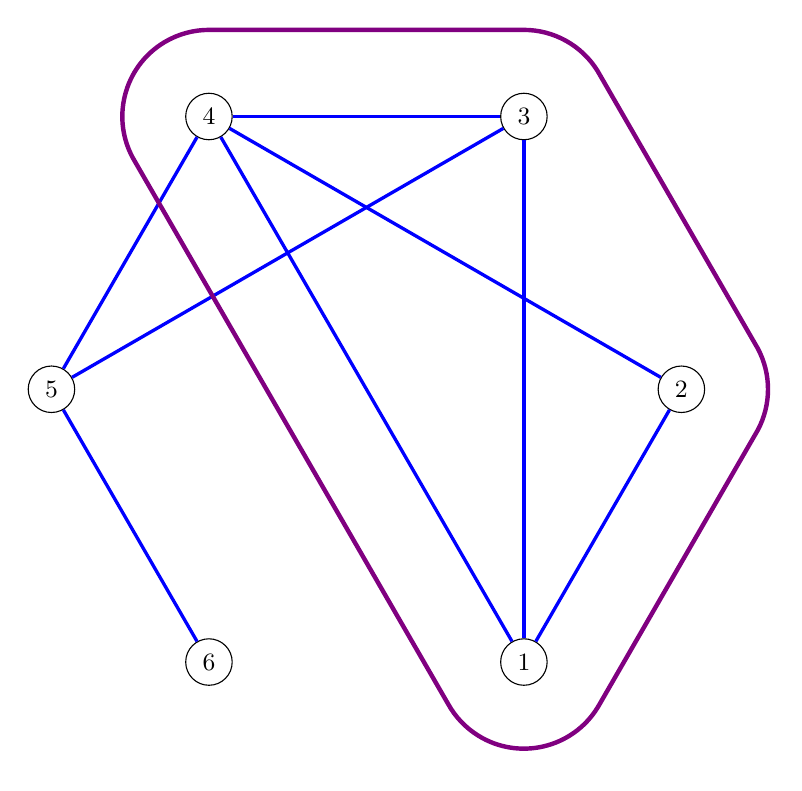
\begin{tikzpicture}
\def \n {6}
\def \radius {4cm}
\def \margin {8} % margin in angles, depends on the radius
\foreach \s in {1,...,6}
{
{\node[draw, circle] (\s) at ({360/\n * (\s - 2)}:\radius)  {\small $\s$};}
} 
\draw [color=blue,very thick] (1) -- (2) ; 
\draw [color=blue,very thick] (4) -- (2) ; 
\draw [color=blue,very thick] (1) -- (3) ; 
\draw [color=blue,very thick] (1) -- (4) ; 
\draw [color=blue,very thick] (4) -- (5) ; 
\draw [color=blue,very thick] (3) -- (5) ; 
\draw [color=blue,very thick] (6) -- (5) ; 
\draw [color=blue,very thick] (3) -- (4) ; 

 % \draw[green,ultra thick] \convexpath{1,5,4,3,2}{1.4cm};
% \draw[yellow,very thick] \convexpath{1,6, 4,3,2}{1.7cm};
\draw[violet,ultra thick] \convexpath{1,4,3,2}{1.1cm};
\end{tikzpicture}} &
\fbox{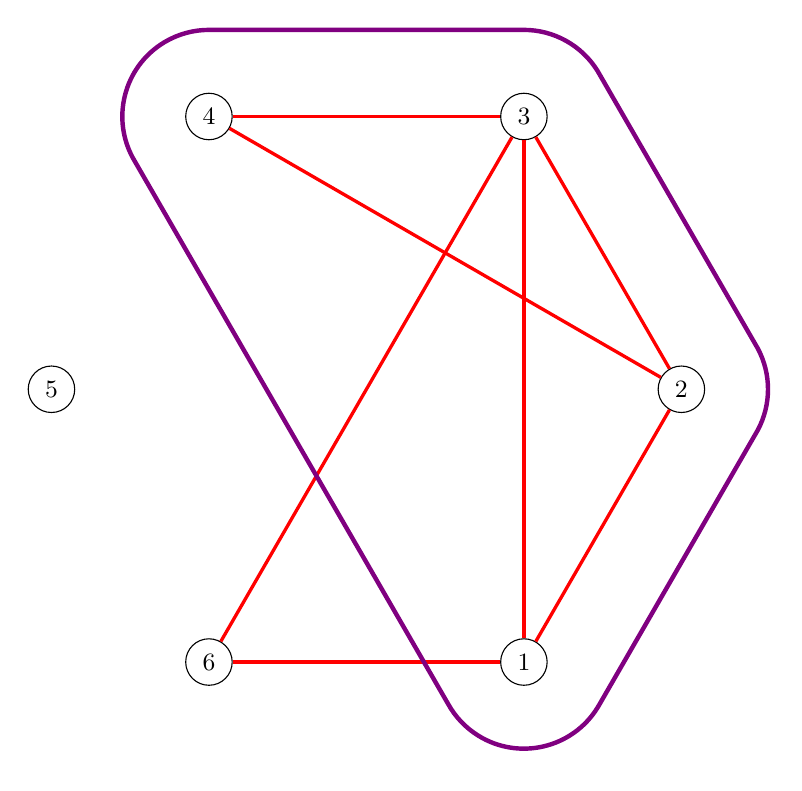
\begin{tikzpicture}
\def \n {6}
\def \radius {4cm}
\def \margin {8} % margin in angles, depends on the radius
\foreach \s in {1,...,6}
{
\node[draw, circle] (\s) at ({360/\n * (\s - 2)}:\radius) {\small $\s$};
} 
\draw [color=red,very thick] (1) -- (2)  ; %node [near end, below=5pt] {\Large\textcolor{red}{$x^{(2)}_{12}$}}; 
\draw [color=red,very thick] (3) -- (2)  ; % node [near end, above=10pt] {\Large\textcolor{red}{$x^{(2)}_{23}$}}; 
\draw [color=red,very thick] (1) -- (3)  ; % node [midway, below=10pt] {\Large\textcolor{red}{$x^{(2)}_{13}$}}; 
\draw [color=red,very thick] (4) -- (2)  ; % node [near start, below=2pt] {\Large\textcolor{red}{$x^{(2)}_{24}$}}; 
\draw [color=red,very thick] (3) -- (4)  ; % node [midway, above=1pt] {\Large\textcolor{red}{$x^{(2)}_{34}$}}; 

\draw [color=red,very thick] (1) -- (6)  ; % node [midway, below=1pt] {\Large\textcolor{red}{$x^{(2)}_{16}$}}; 
\draw [color=red,very thick] (3) -- (6)  ; % node [midway, below=2pt] {\Large\textcolor{red}{$x^{(2)}_{36}$}}; 
%  \draw[green,ultra thick] \convexpath{1,5,4,3,2}{1.4cm};
% \draw[yellow,very thick] \convexpath{1,6, 4,3,2}{1.7cm};
\draw[violet,ultra thick] \convexpath{1,4,3,2}{1.1cm};
\end{tikzpicture}} & 

\raisebox{0.4\totalheight}{\parbox[t]{0.3\linewidth}{\begin{tabular}[c]{l|ll|l }
       \hline $S$ & \textcolor{blue}{$\delta^{(1)}$} & \textcolor{red}{$\delta^{(2)}$} & $\delta^{\min}$  \\\hline 
 {123456} & $1.33$ & $1.17$ & $1.17$\\        
\textcolor{black}{12345} & $1.4$ & $1.0$   & $1.0$\\ 
\textcolor{black}{$12346$} & $1.0$ & $1.4$  & $1.0$\\  
     \textcolor{violet}{$1234$} & $1.25$ & $1.25$    & $1.25$ \\
{$\vdots$} & $\vdots$ & $\vdots$  & $\vdots$\\ \hline
\multicolumn{3}{r}{$\delta_{DCS} = $} & $1.25$
\end{tabular}
% \begin{align*} \delta_{DCS} & = \max \delta^{\min}(S) \end{align*}
}} 
\end{tabular}

\end{center}
}

% \setbeamercolor*{thcolor}{fg=tangocolordarkskyblue}

% \makeatletter
% \setbeamertemplate{theorem begin}
%   {\usebeamercolor[fg]{thcolor}% for the heading
%   {\bfseries\inserttheoremname~}%
%   \ifx\inserttheoremaddition\@empty\else(\inserttheoremaddition)\ \fi%
%   \hspace{.01em}\normalfont\usebeamercolor[fg]{thcolor}% for the body
%   }
% \setbeamertemplate{theorem end}{}
% \makeatother


% document properties
\title{\Huge Finding dense subgraphs in relational graphs}
\author{Vinay Jethava, Niko Beerenwinkel}

\institute{{\tt vinay.jethava@bsse.ethz.ch, niko.beerenwinkel@bsse.ethz.ch}}

\newcommand{\alert}[1]{\textcolor{red}{#1}}
%------------------------------------------------------------------------------
\begin{document}

\begin{frame}{}
\begin{columns}[t]


%-----------------------------------------------------------------------------
%                                                                     COLUMN 1
% ----------------------------------------------------------------------------
\column{0.3}

\block{Coherent sub-networks in genome-scale metabolic models}{
\begin{center}
\begin{tabular}{cc}
\begin{tabular}[c]{ccc}
% 
\includegraphics[height=0.05\textheight]{metabolic-images/p1}  & 
\includegraphics[height=0.035\textheight]{metabolic-images/genotype}  &  \nwA \\
patient & mutations & metabolic model \\ 

\includegraphics[height=0.05\textheight]{metabolic-images/p2} & 
\includegraphics[height=0.05\textheight]{metabolic-images/genotype} & \fbox{\nwB}\\ 

\includegraphics[height=0.05\textheight]{metabolic-images/p3} & 
\includegraphics[height=0.05\textheight]{metabolic-images/genotype} & \fbox{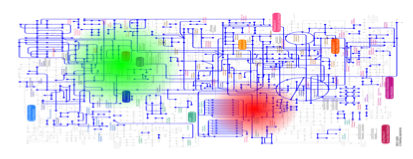
\includegraphics[width=0.3\linewidth]{metabolic-images/nw2}}
\end{tabular} &
\parbox{0.3\linewidth}{
{\small \url{http://www.metabolicatlas.org/}}
\begin{itemize}
\item $917$ patients
\item $|V| \sim 4000$
\item $|E| \sim 15000$
\end{itemize}

} 
\end{tabular}
\end{center}
\begin{description}
\item[{\Large Aim}] {Find {\bf dense common subgraphs} in patients with specific markers e.g. $mutbrca = 1$ and $mutp53 = 1$} 
\item[]
\item[] \alert{Existing methods do not scale  [\cite{jiang2009mining,li2011integrative}]} 
% \begin{itemize}
% \item Exhaustive enumeration
% \item Relaxation of non-convex optimization 
% \end{itemize}
\end{description}
} 

% \begin{block}{Dense Common Subgraph~({\tt DCS}) problem}
% \begin{description}       
% \item[{\tt DCS}] Given relational graph set $G^{(1)} = (V, E^{(1)})$, $G^{(2)} = (V, E^{(2)}), \ldots$, 
% {\[ \delta_{DCS} = \max_{S\subseteq V} \min_{ G^{(m)} }  \frac{ \#\{\text{edges induced by } S      \text{ in } G^{(m)} \} }{|S|}  \]}
% \item[Example]
% \end{description}

% \begin{center}
% \begin{tabular}{ccc}
% \fbox{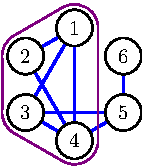
\includegraphics[height=0.225\linewidth]{graphset-images/GA-figure4}} &
% \fbox{
\includegraphics[height=0.225\linewidth]{graphset-images/GB-figure4}} &
% \raisebox{0.45\totalheight}{\parbox[t]{0.3\linewidth}{\small \begin{tabular}[c]{l|ll|l }
%        \hline $S$ & \textcolor{blue}{$\delta^{(1)}$} & \textcolor{red}{$\delta^{(2)}$} & $\delta^{\min}$  \\\hline 
%  {123456} & $1.33$ & $1.17$ & $1.17$\\        
% \textcolor{black}{12345} & $1.4$ & $1.0$   & $1.0$\\ 
% \textcolor{black}{$12346$} & $1.0$ & $1.4$  & $1.0$\\  
%      \textcolor{violet}{$1234$} & $1.25$ & $1.25$    & $\mathbf{1.25}$ \\
% {$\vdots$} & $\vdots$ & $\vdots$  & $\vdots$\\ \hline
% \multicolumn{3}{r}{$\delta_{DCS} = $} & $1.25$
% \end{tabular}
% }} 
% \end{tabular}
% \end{center}
% % \dcsexample
% \end{block}

% %     % MAP problem
% % \begin{exampleblock}{Common Dense Subgraph problem}
% %        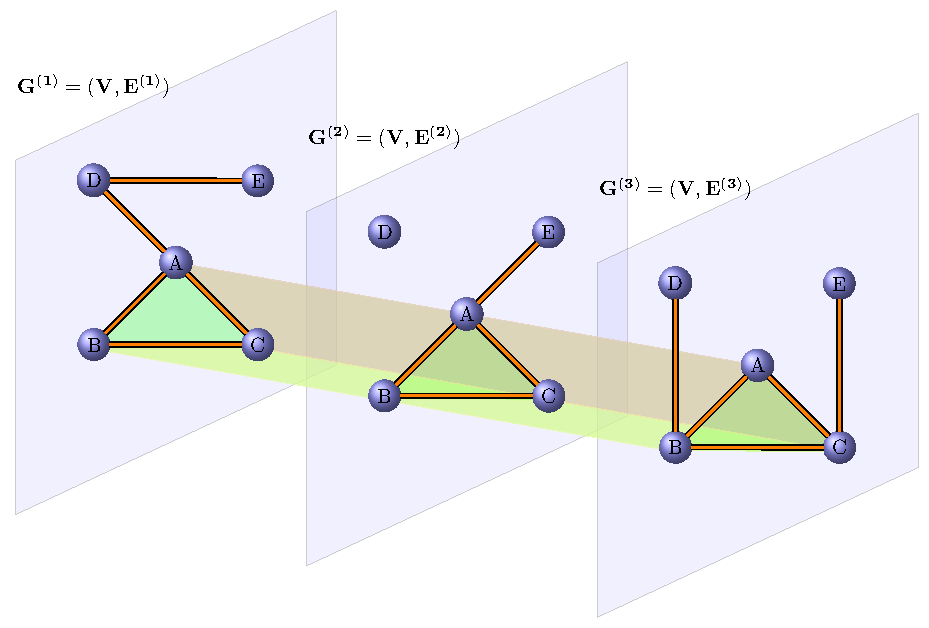
\includegraphics[width=\linewidth]{figures/rw2}
% % {\Large
% % \[ \delta_{CDS} = \max_{S\subseteq V} \min_{ G^{(m)} }  \frac{ \#\{\text{edges induced by } S      \text{ in } G^{(m)} \} }{|S|}  \]
% % }

% % \end{exampleblock}

% \begin{block}{Background: Charikar's algorithm for Dense Subgraph}
% If single graph, {\tt DCS} is equivalent to Dense Subgraph problem, 
% \[ \delta = \max_{S\subseteq V} \frac{|E(S)|}{|S| }\]
% \begin{itemize}
% \item Exact solution [\cite{GoldbergG84,charikar2000greedy}]
% \begin{center}
% \begin{tabular}{lr}
% \fbox{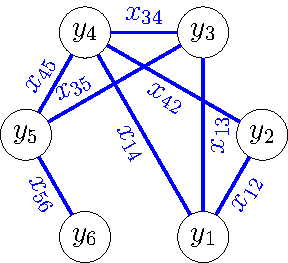
\includegraphics[height=0.2\linewidth]{graphset-images/GA-LP-single}} &
% \raisebox{0.45\totalheight}{\parbox{0.5\linewidth}{
% { \[\begin{array}{rll} 
% \delta = \max_{x, y} & \sum_{ij\in E}   x_{ij}  \\
% s.t. \; & \sum_{i} y_{i} \le 1 \\ 
% &   x_{ij} \le \min (y_{i}, y_{j})  & \forall ij \in E\\ 
% & x_{ij} \ge 0, y_{i} \ge 0 
% \end{array} \]  } 
% % \begin{itemize}
% % \item \alert{LP Opt. ($\sum_{ij} x^{*}_{ij}$)= $\delta$} 
% % \item \alert{$S = \{ i : y_{i}^{*} > 0 \}$}
% % \end{itemize}
% } } 
% \end{tabular}
% \end{center}
% \item Greedy 2-approximation: {\tt repeatedly remove least degree node and return subgraph with highest average degree} 
% \end{itemize}
% \begin{tabular}{cccclrr}
% & 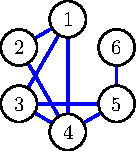
\includegraphics[height=0.15\linewidth]{graphset-images/GA-figure0} 
% & 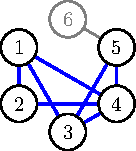
\includegraphics[height=0.15\linewidth]{graphset-images/GA-figure1}  
% &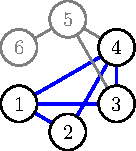
\includegraphics[height=0.15\linewidth]{graphset-images/GA-figure3}   & $\ldots$\qquad \qquad & 
% \tikz \node[fill=tangocolorlightaluminium] {\Large $\delta_{opt} \le  2 \delta_{greedy}$}; \\
% $\delta$: & $1.33$ & $\mathbf{1.40}$  & $1.25$ & $\ldots $
% \end{tabular}
% \end{block}



% %-----------------------------------------------------------------------------
% %                                                                     COLUMN 2
% % ----------------------------------------------------------------------------
% \begin{column}{0.3\linewidth}
% \begin{block}{{\tt DCS\_LP} Linear Program for Dense Common Subgraph}
% \begin{tabular}{ccl}
% \textcolor{blue}{$G^{(1)}$} & \textcolor{red}{$G^{(2)}$} & {\tt DCS\_LP}\\ 
% \fbox{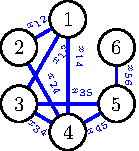
\includegraphics[width=0.25\linewidth]{graphset-images/dcs-lp-figure0}} & 
% \fbox{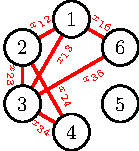
\includegraphics[width=0.25\linewidth]{graphset-images/dcs-lp-figure1}} &
% \raisebox{0.5\totalheight}{ $ \begin{array}{lll} 
% \multicolumn{2}{l}{\max_{x, y, t} \; t} \\ 
%  \;\; &   \sum_{ij\in E^{(m)}} x^{(m)}_{ij} \ge t  & {\small \forall G^{(m)} } \\
% & x^{(m)}_{ij} \le \min (y_{i}, y_{j})   &{\small \forall ij\in E^{(m)} }\\
% & \sum_{i} y_{i} \le 1 \\ 
% & x^{(m)}_{ij} \ge 0, y_{i} \ge 0 
% \end{array}$}
% \end{tabular}
% \end{block}

% \begin{block}{How good is {\tt DCS\_LP} -- Is $t^{*}= \delta_{DCS}$? Can one recover optimal $S_{DCS}$ from LP solution?} 
% % \begin{lemma}{If $y^{*} = \frac{1}{r} \, [ \underbrace{1, \ldots, 1}_{r}, 0, \ldots, 0]$, then $t^{*} = \delta_{DCS}$  and $S_{DCS} = \{i : y_{i}^{*} > 0\}$} 
% % \end{lemma}
% \tikz \node [fill=tangocolorlightaluminium] {If { $y^{*} = [ \underbrace{\frac{1}{n}, \ldots, \frac{1}{n}}_{\Large  n}, 0, \ldots, 0]$}, then $t^{*} = \delta_{DCS}$  and  $S_{DCS} = \{i : y_{i}^{*} > 0\}$}; 

% \begin{center}
% % \parbox{0.3\linewidth}{
% \tikz \node [fill=tangocolorlightplum] {\Large No in general!}; 
%  {
%  \begin{itemize}
% \item Integrality gap $\delta_{DCS} < t^{*}$
% \item Cannot always recover $S_{DCS}$ from LP solution 
% \end{itemize}
% }
% %  }

% \begin{tabular}[c]{ccc}
% % \begin{tabular}{c} 
% \\ 
% \begin{tabular}{cc}
% 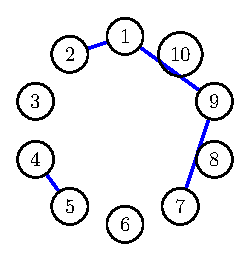
\includegraphics[width=0.225\linewidth]{graphset-images/dcs-lp-figure2} & 
% 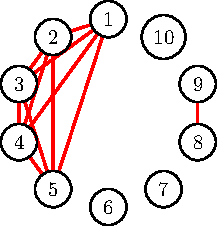
\includegraphics[width=0.225\linewidth]{graphset-images/dcs-lp-figure3}  \\
% \multicolumn{2}{c}{\tikz \node [fill=tangocolorlightaluminium] {$\delta_{DCS} = 0.67$, $t^{*}  = 0.7$};} 
% \end{tabular}
% & \begin{tabular}{c}
% 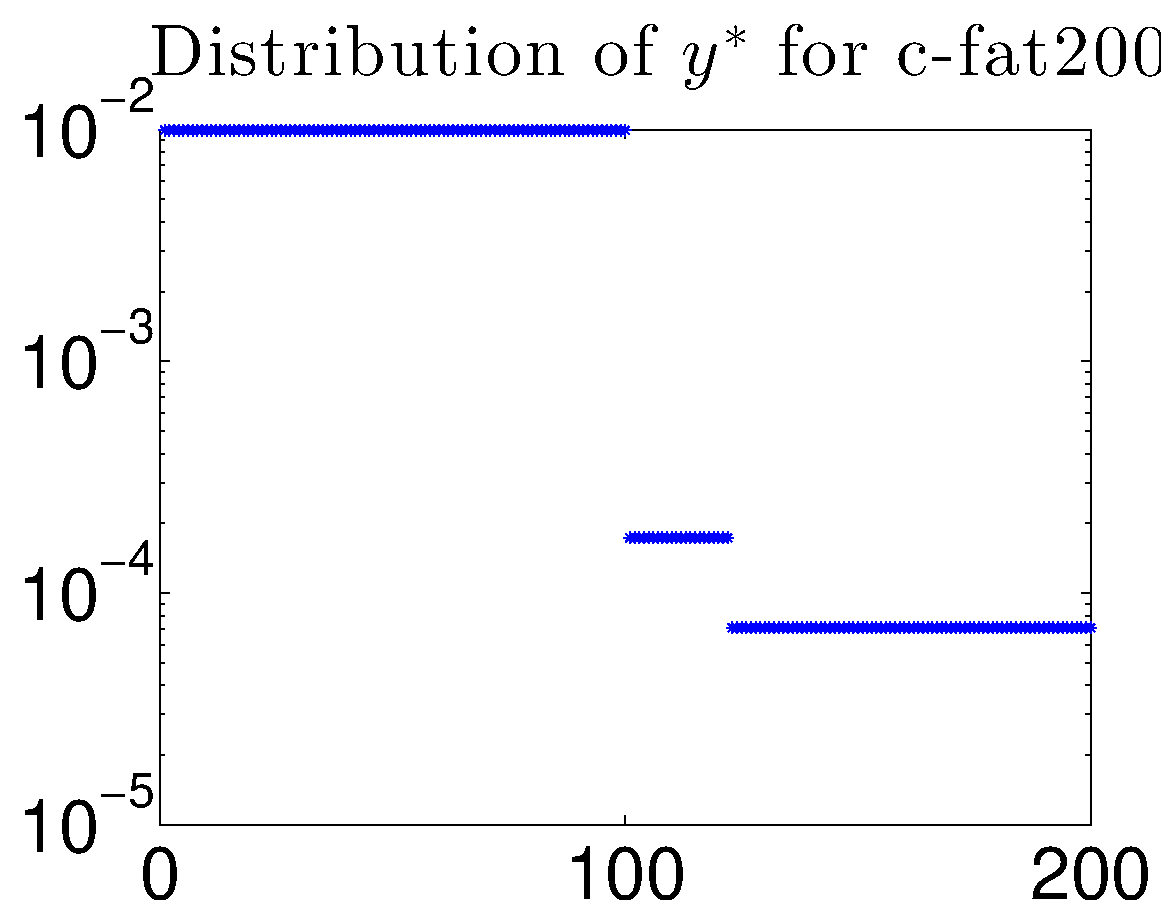
\includegraphics[width=0.325\linewidth]{images/cds/y-cfat200} \\ \tikz \node [fill=tangocolorlightaluminium] {$S_{DCS} \neq \{ i: y_{i}^{*}  > 0 \} $}; 
% \end{tabular}
% \end{tabular}
% \end{center}

% \end{block}

% \begin{block}{Greedy algorithm for {\tt DCS}}
% {\large
% \begin{enumerate}
% \item Choose least dense graph in relational graph set
% \item Find minimum degree node in the least dense graph
% \item Remove node from graph set and repeat $1-3$. 
% \end{enumerate}
% }
% \begin{tabular}{cc}
% \begin{tabular}[c]{ccccccc}
% % $\delta^{(1)}$ & $1.33$ & {\bf $1.0$}& $1.25$ &\\ 
%  & \fbox{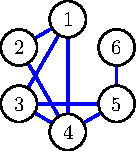
\includegraphics[width=0.175\linewidth]{graphset-images/GA-figure0}}
% & \fbox{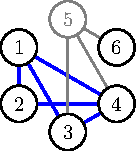
\includegraphics[width=0.175\linewidth]{graphset-images/GA-figure2}}
% & \fbox{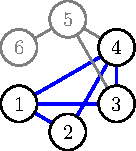
\includegraphics[width=0.175\linewidth]{graphset-images/GA-figure3}}
%  \\ 
% % $\delta^{(2)}$ & {\bf $1.17$} & $1.4$ & $1.25$ & \\ 
% & \fbox{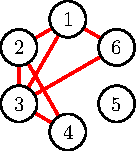
\includegraphics[width=0.175\linewidth]{graphset-images/GB-figure0}}
% & \fbox{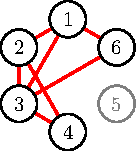
\includegraphics[width=0.175\linewidth]{graphset-images/GB-figure2}}
% & 
% \fbox{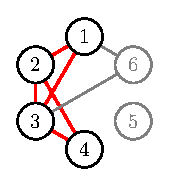
\includegraphics[width=0.175\linewidth]{graphset-images/GB-figure3}}  \\
% \end{tabular}
% &
% \begin{tabular}{|cc|c|}
% \hline 
% \textcolor{blue}{$\delta^{(1)}$} & \textcolor{red}{$\delta^{(2)}$} & $v_{remove}$ \\\hline
% $1.33$ & $1.17$ & {\textcolor{red}{$5$}} \\
% {$1.0$ } &  {$1.4$ } &  {\textcolor{blue}{$6$}} \\  
% {$1.25$ } &  {$1.25$ } & {\textcolor{blue}{$2$}}  \\  
% {$1.0$} & {$0.67$} & {\textcolor{red}{$4$}} \\
% {$0.5$} & {$0.5$} & {\textcolor{blue}{$3$}} \\\hline
% \multicolumn{3}{c}{{$\delta_{dcs\_greedy} = 1.25$}}
% \end{tabular}
% \end{tabular}
% \end{block}


% \end{column}

% %-----------------------------------------------------------------------------
% %                                                                     COLUMN 3
% % ----------------------------------------------------------------------------
% \begin{column}{.30\linewidth}

% % \begin{block}{How good is {\tt DCS\_GREEDY}?}


% % \begin{center}
% % \begin{tabular}[c]{cccc}
% %  \fbox{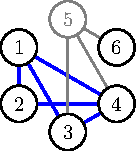
\includegraphics[width=0.175\linewidth]{graphset-images/GA-figure2}}
% % & \fbox{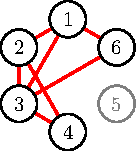
\includegraphics[width=0.175\linewidth]{graphset-images/GB-figure2}}
% % & \fbox{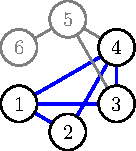
\includegraphics[width=0.175\linewidth]{graphset-images/GA-figure3}}
% % & \fbox{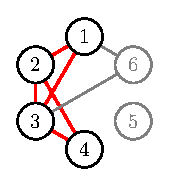
\includegraphics[width=0.175\linewidth]{graphset-images/GB-figure3}}\\  \\
% % \end{tabular}

% % \begin{tabular}{cc}
% %  \begin{tabular}[c]{cc|c|ccc|c}\hline 
% %  \textcolor{blue}{$\delta^{(1)}$} & \textcolor{red}{$\delta^{(2)}$} &  {$v_{remove}$} & $\underline{n}$ & $\underline{d} $ &$\hat{d}$ & $r$\\ \hline
% % % % ~\footnote{$r = \frac{d_{max} n}{\underline{d}\underline{n}}$}\\\hline
% %  {$1.33$} & {$\underline{1.17}$} &   {\textcolor{red}{$5$}}  & {\textcolor{red}{5}} & {\textcolor{red}{2}} & {\textcolor{blue}{3}} & $1.8$ \\
% %  {$\underline{1.0}$ } &  {$1.4$} & {\textcolor{blue}{$6$}} & {\textcolor{blue}{4}} & {\textcolor{blue}{2}}&  {\textcolor{red}{2}} & $1.25$\\  \hline     
% %  \end{tabular} & 
% % \tikz \node [fill=tangocolorlightaluminium]  {\Large $ \delta_{DCS} \le 2 r_{\max} \delta_{\tt GREEDY}$ }; 
% % \end{tabular}

% % \end{center}
% % \end{block}

% \begin{block}{How good is {\tt DCS\_GREEDY}?}
% \begin{center}
% \begin{tabular}{cc}
% \begin{tabular}[c]{ccccccc}
% % $\delta^{(1)}$ & $1.33$ & {\bf $1.0$}& $1.25$ &\\ 
% & \fbox{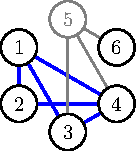
\includegraphics[width=0.15\linewidth]{graphset-images/GA-figure2}}
% & \fbox{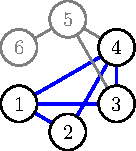
\includegraphics[width=0.15\linewidth]{graphset-images/GA-figure3}}
%  \\ 
% % $\delta^{(2)}$ & {\bf $1.17$} & $1.4$ & $1.25$ & \\ 
% & \fbox{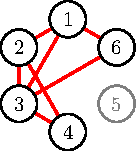
\includegraphics[width=0.15\linewidth]{graphset-images/GB-figure2}}
% & \fbox{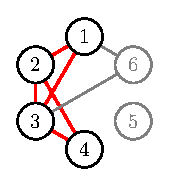
\includegraphics[width=0.15\linewidth]{graphset-images/GB-figure3}}  \\
% \end{tabular}
% &
% % \begin{parbox}{0.5\linewidth}{
%  \begin{tabular}[c]{cc|c|ccc|c}\hline 
%  \textcolor{blue}{$\delta^{(1)}$} & \textcolor{red}{$\delta^{(2)}$} &  {$v_{remove}$} & $\underline{n}$ & $\underline{d} $ &$\hat{d}$ & $r$\\ \hline
% % % ~\footnote{$r = \frac{d_{max} n}{\underline{d}\underline{n}}$}\\\hline
%  {$1.33$} & {$\underline{1.17}$} &   {\textcolor{red}{$5$}}  & {\textcolor{red}{5}} & {\textcolor{red}{2}} & {\textcolor{blue}{3}} & $1.8$ \\
%  {$\underline{1.0}$ } &  {$1.4$} & {\textcolor{blue}{$6$}} &     {\textcolor{blue}{4}} & {\textcolor{blue}{2}}&  {\textcolor{red}{2}} & $1.25$\\  
% $\vdots$ & $\vdots$               &  $\vdots$                   & $\vdots$ &                                     $\vdots$ & $\vdots$ & $\vdots$ \\  \hline
%   \\
%    \multicolumn{7}{c}{\tikz \node [fill=tangocolorlightaluminium]  {\Large $ \delta_{DCS} \le 2 r_{\max} \delta_{\tt GREEDY}$ } ; } 
%  \end{tabular}


% % }
% \end{tabular}

% \end{center}
% \end{block}


% \newcommand{\gsq}{\textcolor{green}{$\blacksquare$}}
% \newcommand{\ysq}{\textcolor{yellow}{$\blacksquare$}}
% \newcommand{\rsq}{\textcolor{red}{$\blacksquare$}}
% \newcommand{\bsq}{{$\blacksquare$}}

% \begin{block}{Results on DIMACS and SNAP graph sets}
% \begin{center}
% \begin{tabular}[c]{cc}
% 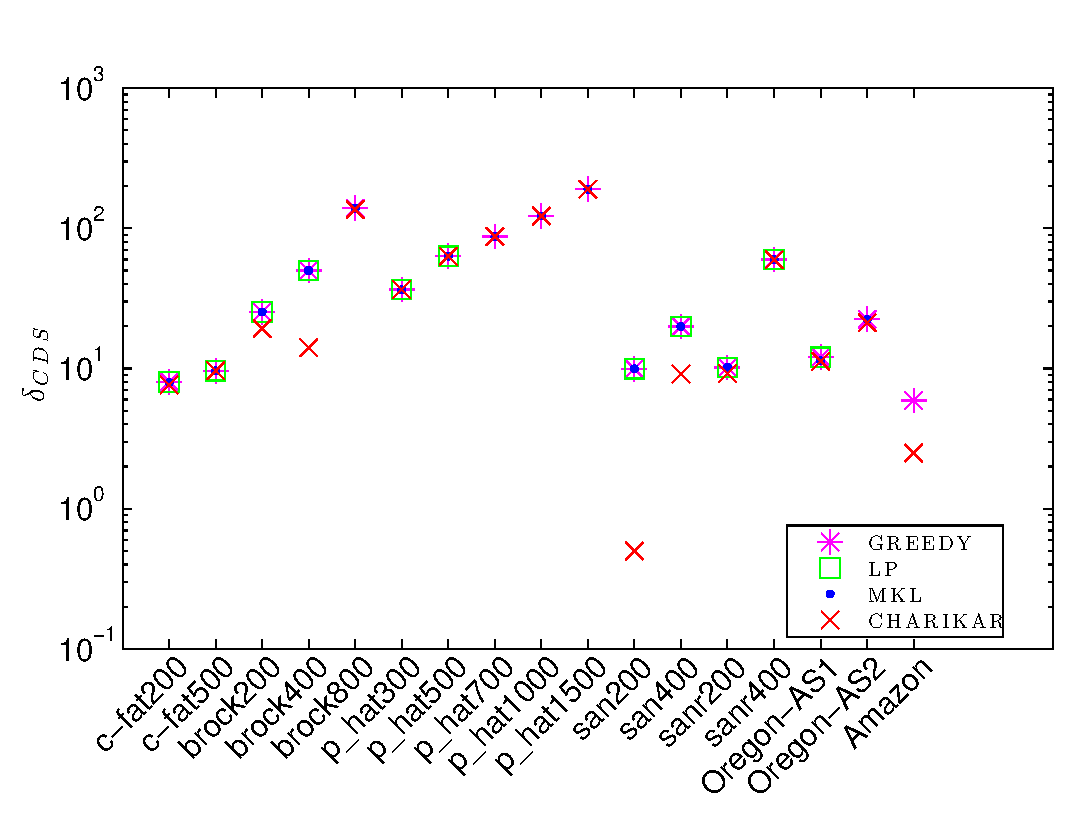
\includegraphics[width=0.5\linewidth]{images/cds/delta-cds} &
% \raisebox{0.5\totalheight}{ \tiny
% \begin{tabular}[c]{rrrr}\hline%
% $\GG$& $n$ &$n_{\GG}$&LP\\\hline
% {c-fat200} (3)&200&13242&\rsq\\
% {c-fat500} (4)&500&83416&\gsq\\
% {brock200} (4)&200&29753&\gsq\\
% {brock400} (4)&400&80245&\gsq\\
% {brock800} (4)&800&447753&\bsq\\
% {p\_hat300} (3)&300&66251&\gsq\\
% {p\_hat500} (3)&500&188315&\gsq\\
% {p\_hat700} (3)&700&365737&\bsq\\
% {p\_hat1000} (3)&1000&738798&\bsq\\
% {p\_hat1500} (3)&1500&1701127&\bsq\\
% {san200} (5)&200&17910&\gsq\\
% {san400} (3)&400&119700&\gsq\\
% {sanr200} (2)&200&8069&\gsq\\
% {sanr400} (2)&400&63747&\gsq\\\hline
% {AS1} (9)&11492&203127&\gsq\\
% {AS2} (9)&11806&284031&\bsq\\
% {Amazon} (3)&400727&7157921&\bsq\\\hline 
% \end{tabular} 
% }
% \end{tabular}
% \end{center}
% \begin{itemize} 
% \item LP solution: \gsq=optimal, \rsq=sub-optimal, \bsq=out of time
% \end{itemize}
% \end{block}

% \begin{block}{Subnetworks in  genome-scale metabolic models}
% \begin{itemize}
% \item Dense common subnetworks for specific markers
% \item Method captures altered metabolic pathways
% \end{itemize}
% \begin{center}
% \adjustbox{clip,center}{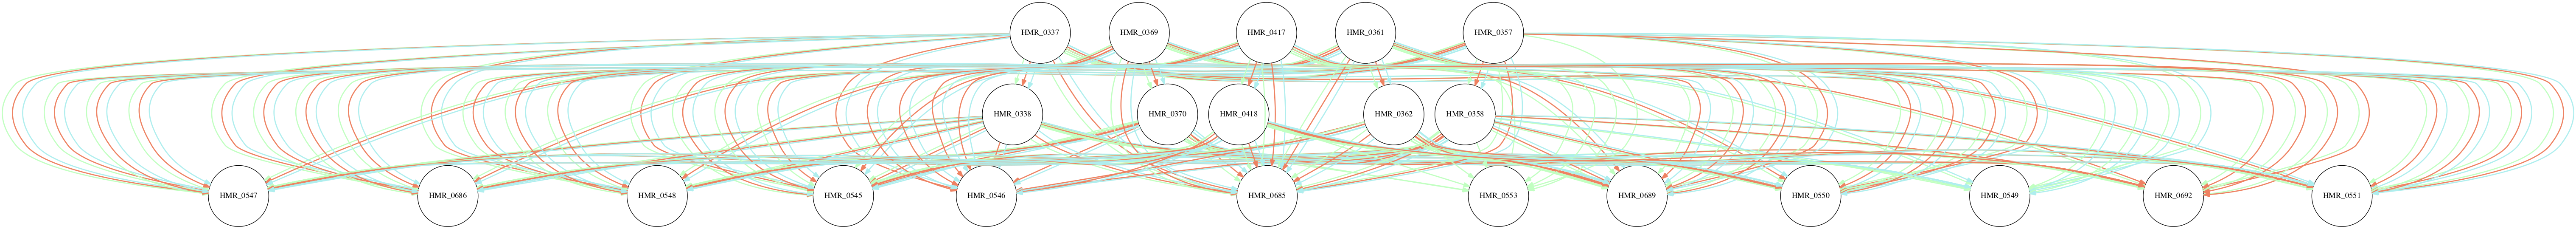
\includegraphics[width=\linewidth]{metabolic-images/svm_clique3} }
% \end{center}
% % \begin{tabular}{cc}
% % 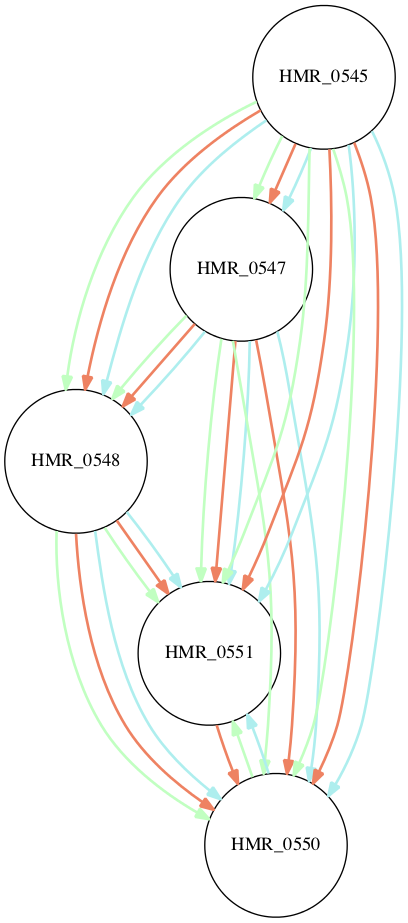
\includegraphics[width=0.1\linewidth]{metabolic-images/svm_clique1}  & 
% % \raisebox{0.5\totalheight}{\parbox{0.9\linewidth}{\begin{itemize}
% % \item Dense common subnetworks for specific markers
% % \item Method captures altered metabolic pathways
% % \item[]
% % \end{itemize}
% % \begin{center}
% % \adjustbox{clip,center}{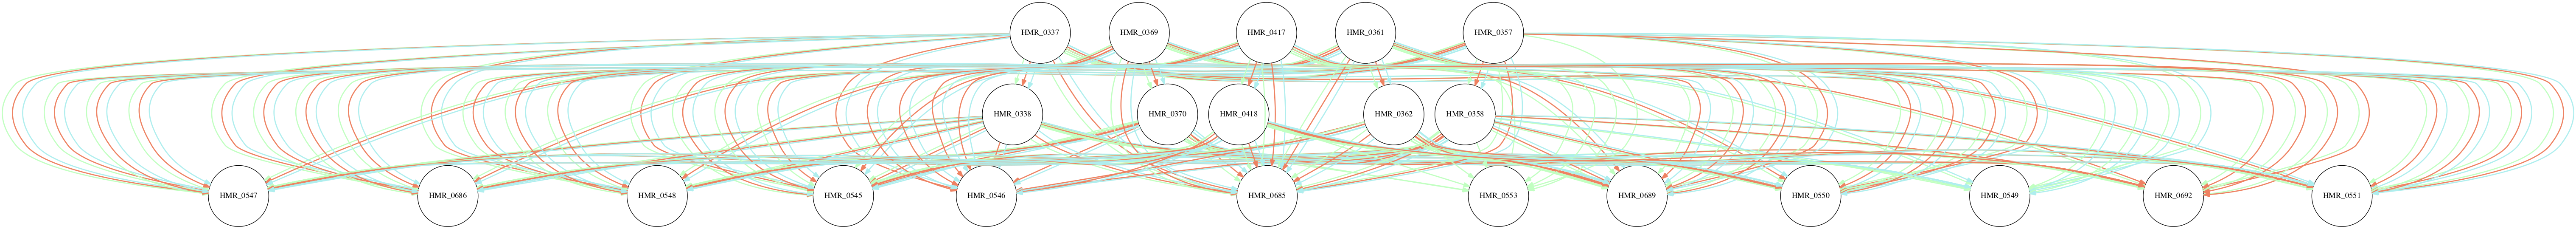
\includegraphics[width=0.85\linewidth]{metabolic-images/svm_clique3} }
% % \end{center}
% % }}
% % \end{tabular}
% \end{block}

% \begin{block}{Summary}
% \begin{itemize}
% \item Extension of Charikar's algorithm to DCS 
% \item LP solution optimal if  $y^{*} = \frac{1}{n} \, [ \underbrace{1, \ldots, 1}_{n}, 0, \ldots, 0]$ 
% \item {\tt DCS\_GREEDY} gives graph-dependent bounds
% \end{itemize}
% \end{block}

% % \begin{block}{Results}  
% % {\tiny\begin{tabular}{|r|r|r|r|r|r|r|r|r|r|r|}\hline
% %  $\GG$	      & \multicolumn{2}{c}{\tt MKL}   & \multicolumn{3}{|c}{\tt LP} & \multicolumn{2}{|c}{\tt GREEDY} & \multicolumn{3}{|c|}{\tt CHARIKAR}    \\  \hline \hline 
% %    &  $|S|$ & $\dg(S)$ &  $|S|$ & $\dg(S)$ & $t^{*}$ & $|S|$ & $\dg(S)$  & $|S|$ & $\dg(S)$ & $\delta_{\cap}(S)$\\ \hline  
% % {\em c-fat200}&100&7.93&101&8.0099&8.0822&102&8.0392 & 199 &         7.6281   & 1.8141 \\
% % {\em c-fat500}&140&9.65&140&9.65&9.65&140&9.65  &140& 9.65  &  9.6500 \\
% % {\em brock200}&200&25.33&200&25.33&25.33&200&25.33 &   149 &         19.309  & 1.9262 \\
% % {\em brock400}&400&50.035&400&50.035&50.035&400&50.035  & 110 &         14.082 &  1.2000\\
% % {\em brock800}&800&139.2925&X&X&X&800&139.2925  & 783  &        136.41 & 5.9872 \\
% % {\em p\_hat300}&300&36.4433&286&36.65&36.65 &286&36.65   & 286  &         36.65 &   36.6503 \\
% % {\em p\_hat500}&500&63.138&489&63.2147&63.2147&489&63.2147 & 489   &       63.2147 & 63.2147\\
% % {\em p\_hat700}&700&87.1414&X&X&X&679&87.274 &  679 &         87.274  & 87.2739  \\
% % {\em p\_hat1000}&1000&122.253&X&X&X&973&122.412   &   973 &         122.41  & 122.4121 \\
% % {\em p\_hat1500}& 1500&189.9487&X&X&X&1478&190.053&  1478     &  190.05  &  190.0535 \\
% % {\em san200}&200&9.95&200&9.95&9.95&200&9.95 & 2 &          0.5 & 0.5000 \\
% % {\em san400}&400&19.95&400&19.95&19.95&400&19.95 & 176       &  9.1364 & 0.6648 \\
% % {\em sanr200}&200&10.185&199&10.1859&10.1859&199&10.1859 & 170 &  9.2294 & 3.1706\\
% % {\em sanr400}&400&59.8275&400&59.8275&59.8275&400&59.8275 & 399   &    59.709 & 29.9749 \\\hline \multicolumn{2}{c}{} \\\hline
% % {\em Oregon-1} & 54  & 11.3704 & 76 & 12.0263 & 12.0263 &  76 & 12.0263 & 64 & 11.2812 & 10.0938 \\
% % {\em Oregon-2} & 173 & 22.3468 &  X & X & X & 119
% %       & 22.4538  & 115 & 21.2261 & 17.5739\\ \hline 
% %  \end{tabular}
% %  }  
% % \end{block}

% \begin{block}{References}
% {\small
%   \begin{itemize} 
% \item \fullcite{GoldbergG84}
% \item \fullcite{charikar2000greedy}
% \item \fullcite{jiang2009mining}
% \item \fullcite{li2011integrative}
%   \end{itemize}
% }
% % \bibliographystyle{plainnat}
% % \begin{thebibliography}{2}
% % \bibitem[C] M
% % M~Charikar. ``Greedy approximation algorithms for finding  dense components in a graph.'' In: \emph{APPROX}, 2000
% % \bibitem[KS] S
% % S~Khuller and B~Saha. ``On finding dense subgraphs.''
% %   In: \emph{ICALP}, 2009 
% % \end{thebibliography}
% \end{block}
% \end{column}

\end{columns}

\end{frame}

\end{document}
